\section{Auswertung}
\label{sec:Auswertung}

\subsection{Energieverlust und Reichweite von Alpha-Strahlung}
\begin{table}[H]
  \centering
  \caption{Messreihe bei einem Abstand von $d_1=\qty{6}{\centi\meter}$.}
  \label{tab:tabelle}
  \sisetup{table-format=1.1, per-mode=reciprocal}
  \begin{tblr}{
      colspec = {S[table-format=3.0] S[table-format=4.0] S[table-format=5.0]},
      row{1} = {guard, mode=math},
    }
    \toprule
    p \mathbin{/} \unit{\milli\bar} & \text{channel} &  \text{Pulse}  \\
    \midrule
    0     &  871  &   19898 \\
    50    &  791  &   20435 \\
    100   &  808  &   17321 \\
    150   &  787  &   17543 \\
    200   &  760  &   17198 \\
    250   &  702  &   16791 \\
    300   &  718  &   15904 \\
    350   &  624  &   15343 \\
    400   &  732  &   1604  \\
    450   &  724  &   21    \\
    500   &  726  &   1     \\
    550   &  \text{---}     &   0     \\
    \bottomrule
  \end{tblr}
\end{table}

\begin{figure}[H]
  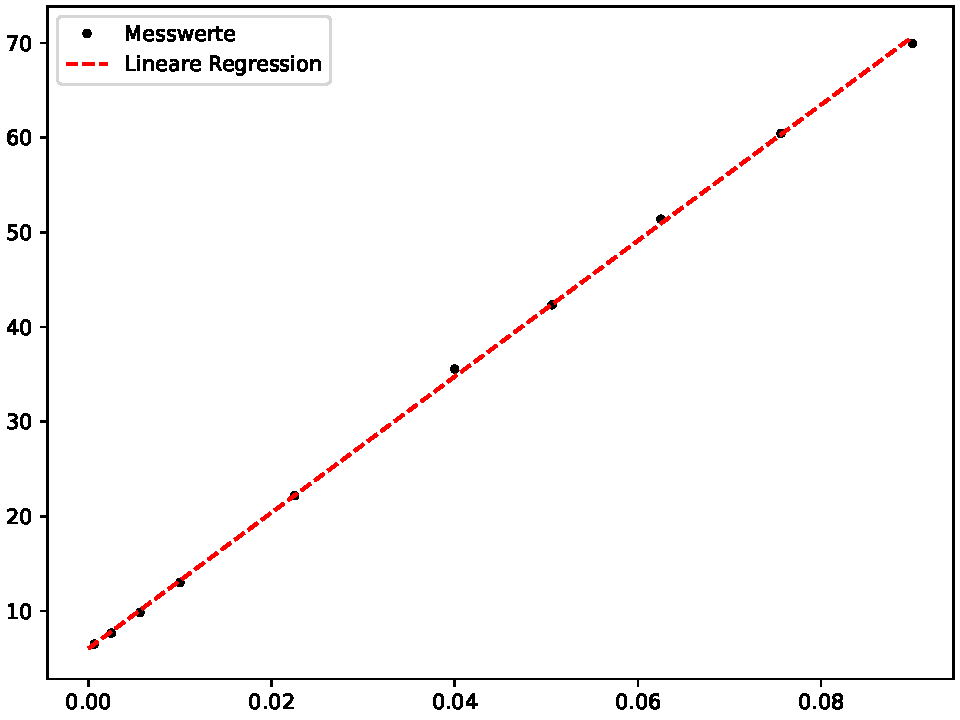
\includegraphics[width=\textwidth]{build/plot.pdf}
  \caption{Die gemessene maximale Energie gegen die effektive Weglänge bei einem Abstand von $d_1=\qty{6}{\centi\meter}$.}
  \label{fig:energie1}
\end{figure}

Über die channel Zahl kann auf die Energie des Teilchens zurückgeschlossen werden, wobei die Teilchen des 
am meisten auftretenden channels, welcher auch immer eingetragen wurde, bei $p=\qty{0}{\bar}$ eine Energie 
von ungefähr $E=\qty{4}{\mega\electronvolt}$ besitzen. \\
\noindent Der in Abbildung \ref{fig:energie1} eingezeichnete Plot ist hierbei eine Regression der Werte, die 
sich bei dem Starken Abfall der Energie befinden. Somit ist die Steigung des Graphen ein Maß für den Energieverlust
der Alphateilchen. Dieser beträgt hier $\frac{\symup{d}E}{\symup{d}x}=\qty{27.45(7.51)}{\mega\electronvolt\per\meter}$.

\begin{figure}[H]
  \includegraphics[width=\textwidth]{build/plotzähl.pdf}
  \caption{Anzahl Detektierter Teilchen in 2-Minuten Intervallen gegen die effektive Weglänge bei einem Abstand von $d_1=\qty{6}{\centi\meter}$.}
  \label{fig:zaehl1}
\end{figure}

\noindent Die mittlere Reichweite der Alphateilchen entspricht dann dem Wert der Ausgleichsgeraden, der bei der 
Hälfte der maximalen Zählrate erreicht ist, wobei für den Verlauf des Abfallens der Zählrate für dieses kurze 
Intervall angenommen wird, dass dieses dort linear verläuft. Somit ergibt sich für die mittlere Reichweite 
$\bar{x}_1=\qty{0.022}{\meter}$.

\begin{table}[H]
  \centering
  \caption{Messreihe bei einem Abstand von $d_2=\qty{5}{\centi\meter}$.}
  \label{tab:tabelle}
  \sisetup{table-format=1.1, per-mode=reciprocal}
  \begin{tblr}{
    colspec = {S[table-format=3.0] S[table-format=4.0] S[table-format=5.0]},
    row{1} = {guard, mode=math},
    }
    \toprule
    p \mathbin{/} \unit{\milli\bar} & \text{channel} &  \text{Pulse} & \\
    \midrule
    0     &  1023   &  23373  \\
    50    &  919    &  22738  \\
    100   &  875    &  22456  \\
    150   &  877    &  22065  \\
    200   &  847    &  21181  \\
    250   &  847    &  20389  \\
    300   &  787    &  18596  \\
    350   &  727    &  14934  \\
    400   &  727    &  10416  \\
    450   &  726    &  3609   \\
    500   &  725    &  645    \\
    550   &  725    &  87     \\
    600   &  726    &  56     \\
    650   &  725    &  49     \\
    700   &  727    &  25     \\
    750   &  726    &  36     \\
    800   &  724    &  30     \\
    \bottomrule
  \end{tblr}
\end{table}

\begin{figure}[H]
  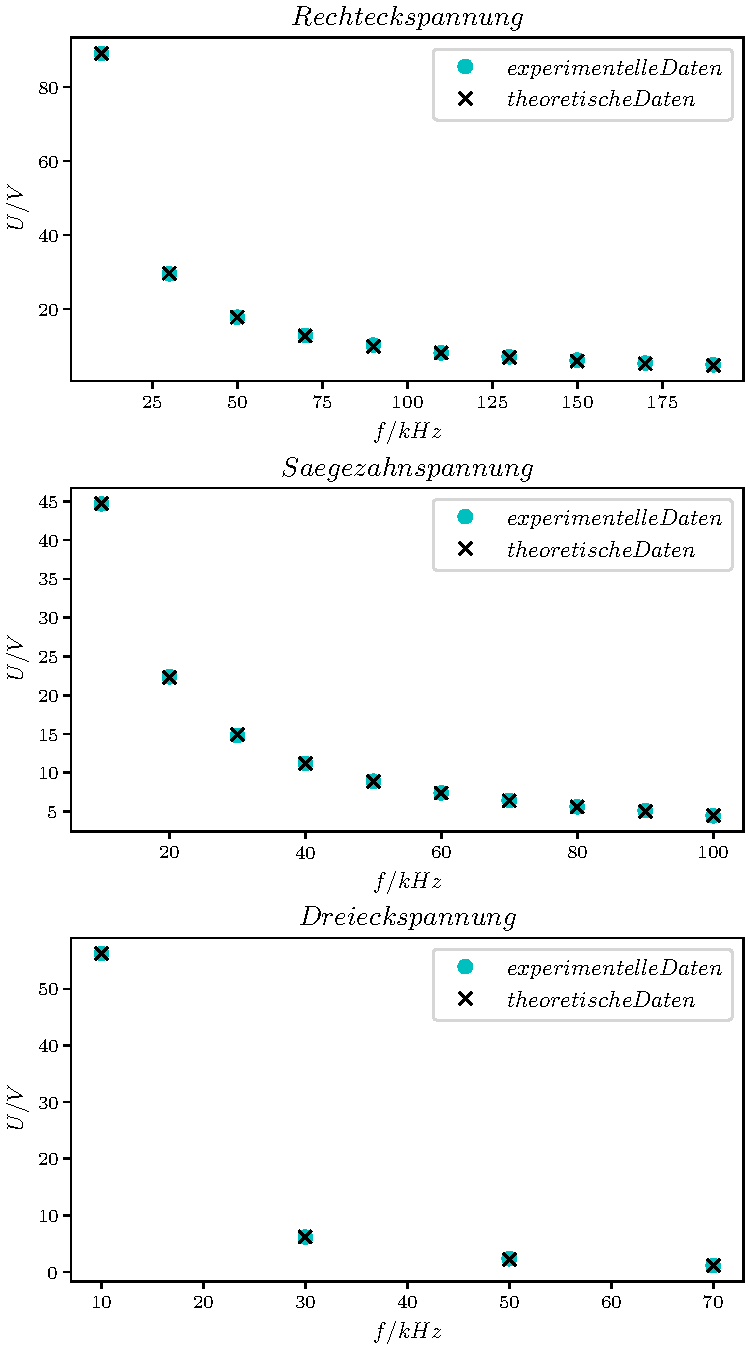
\includegraphics[width=\textwidth]{build/plot1.pdf}
  \caption{Die gemessene maximale Energie gegen die effektive Weglänge bei einem Abstand von $d_2=\qty{5}{\centi\meter}$.}
  \label{fig:energie2}
\end{figure}

Analog zu der Methode der ersten Messreihe ergibt sich hier mithilfe der Abbildung \ref{fig:energie2} 
ein mittlerer Energieverlust von $\frac{\symup{d}E}{\symup{d}}=\qty{44.16(4.83)}{\mega\electronvolt\per\meter}$.

\begin{figure}[H]
  \includegraphics[width=\textwidth]{build/plot1zähl.pdf}
  \caption{Anzahl Detektierter Teilchen in 2-Minuten Intervallen gegen die effektive Weglänge bei einem Abstand von $d_1=\qty{6}{\centi\meter}$.}
  \label{fig:zaehl2}
\end{figure}

Desweiteren folgt mit \ref{fig:zaehl2}, dass die mittlere Reichweite $\bar{x}_2=\qty{0.018(0.003)}{\meter}$ ist.

\subsection{Statistik des Zerfalls}

In der Tabelle \ref{tab:Statistik} ist die Anzahl der Alpha-Teilchen, welche innerhalb von 10 Sekunden auf den Detektor auftreffen, für 100 Durchführungen eingetragen. 



\begin{table}[H]
    \centering
    \caption{In dieser Tabelle sind die Messwerte für die Statistik des Zerfalls aufgeführt. $n$ ist hier die Nummer der Durchführung und $z$ die gemessene Zahl der Alphateilchen.} 
    \label{tab:Statistik}
    %\sisetup{table-format=1.1, per-mode=reciprocal}
    \begin{minipage}[t]{0.2\linewidth}
    \begin{tblr}[t]{
        colspec = {S[table-format=3.0] S[table-format=4.0]},
        row{1} = {guard, mode=math},
      }
      \toprule
      n  & z  \\
      \midrule
        1   &   1768  \\     
        2   &   1777  \\    
        3   &   1892  \\
        4   &   1601  \\
        5   &   1848  \\
        6   &   1721  \\
        7   &   1816  \\
        8   &   1922  \\
        9   &   1855  \\
       10   &   1762  \\
       11   &   1910  \\
       12   &   1845  \\
       13   &   1776  \\
       14   &   1928  \\
       15   &   1892  \\
       16   &   1850  \\
       17   &   1784  \\
       18   &   1874  \\
       19   &   1974  \\
       20   &   1827  \\
       21   &   1773  \\
       22   &   1883  \\
       23   &   1793  \\
       24   &   1711  \\
       25   &   1726  \\
      \bottomrule
    \end{tblr}
  \end{minipage}
  \hfill
  \begin{minipage}[t]{0.2\linewidth}
    \begin{tblr}[t]{
      colspec = {S[table-format=3.0] S[table-format=4.0]},
      row{1} = {guard, mode=math},
    }
    \toprule
    n  & z  \\
    \midrule
    26   &   1891  \\
    27   &   1797  \\
    28   &   1846  \\
    29   &   1817  \\
    30   &   1896  \\
    31   &   1909  \\
    32   &   1803  \\
    33   &   1940  \\
    34   &   1888  \\
    35   &   1895  \\
    36   &   1827  \\
    37   &   1927  \\
    38   &   1754  \\
    39   &   1794  \\
    40   &   1742  \\
    41   &   1759  \\
    42   &   1774  \\
    43   &   1824  \\
    44   &   1957  \\
    45   &   1833  \\
    46   &   1842  \\
    47   &   1903  \\ 
    48   &   1822  \\
    49   &   1842  \\
    50   &   1740  \\
    \bottomrule
  \end{tblr}
\end{minipage}
\hfill
\begin{minipage}[t]{0.2\linewidth}
  \begin{tblr}[t]{
    colspec = {S[table-format=3.0] S[table-format=4.0]},
    row{1} = {guard, mode=math},
  }
  \toprule
  n  & z  \\
  \midrule
  51   &   1873  \\
  52   &   1793  \\
  53   &   1938  \\
  54   &   1776  \\
  55   &   1819  \\
  56   &   1954  \\
  57   &   1926  \\
  58   &   1871  \\
  59   &   1766  \\
  60   &   1846  \\
  61   &   1773  \\
  62   &   1747  \\
  63   &   1753  \\
  64   &   1783  \\
  65   &   1923  \\
  66   &   1828  \\
  67   &   1836  \\
  68   &   1759  \\
  69   &   1772  \\
  70   &   1796  \\
  71   &   1799  \\
  72   &   1827  \\
  73   &   1799  \\
  74   &   1792  \\
  75   &   1784  \\
  \bottomrule
\end{tblr}
\end{minipage}
\hfill
\begin{minipage}[t]{0.2\linewidth}
  \begin{tblr}[t]{
    colspec = {S[table-format=3.0] S[table-format=4.0]},
    row{1} = {guard, mode=math},
  }
  \toprule
  n  & z  \\
  \midrule
  76   &   1822  \\
  77   &   1835  \\
  78   &   1790  \\
  79   &   1691  \\
  80   &   1903  \\
  81   &   1710  \\ 
  82   &   1881  \\
  83   &   1704  \\
  84   &   1894  \\
  85   &   1935  \\
  86   &   1956  \\
  87   &   1836  \\
  88   &   1914  \\
  89   &   1762  \\
  90   &   1868  \\ 
  91   &   1676  \\
  92   &   1772  \\
  93   &   1892  \\
  94   &   1876  \\
  95   &   1757  \\
  96   &   1880  \\
  97   &   1879  \\
  98   &   1870  \\
  99   &   1706  \\
 100   &   1836  \\
  \bottomrule
\end{tblr}
\end{minipage}

\end{table}


  

  Der Mittelwert der Teilchenzahl ist $\bar{z}=1827.08(72.22)$.
  Mit diesem Wert und seiner Standardabweichung kann nun eine Poisson-Verteilung und eine Gauß Verteilung simuliert werden.
  Diese sind in Abbildung \ref{fig:Statistik} aufgezeichnet.
  
  \begin{figure}[H]
    \includegraphics[width=\textwidth]{build/Statistik.pdf}
    \caption{Hier ist die Verteilung der Messwerte in blau, die Poisson-Verteilung in gelb und die Gauß-Verteilung in rot eingezeichnet.
    Dabei ist $z$ die Teilchenzahl und $N$ die Häufigkeit, mit der diese vorkommen.}
    \label{fig:Statistik}
  \end{figure}




